




\section{time analysis}
This section is based on the commit "Interactive with time measurement".

\begin{figure}[h]
	\centering
	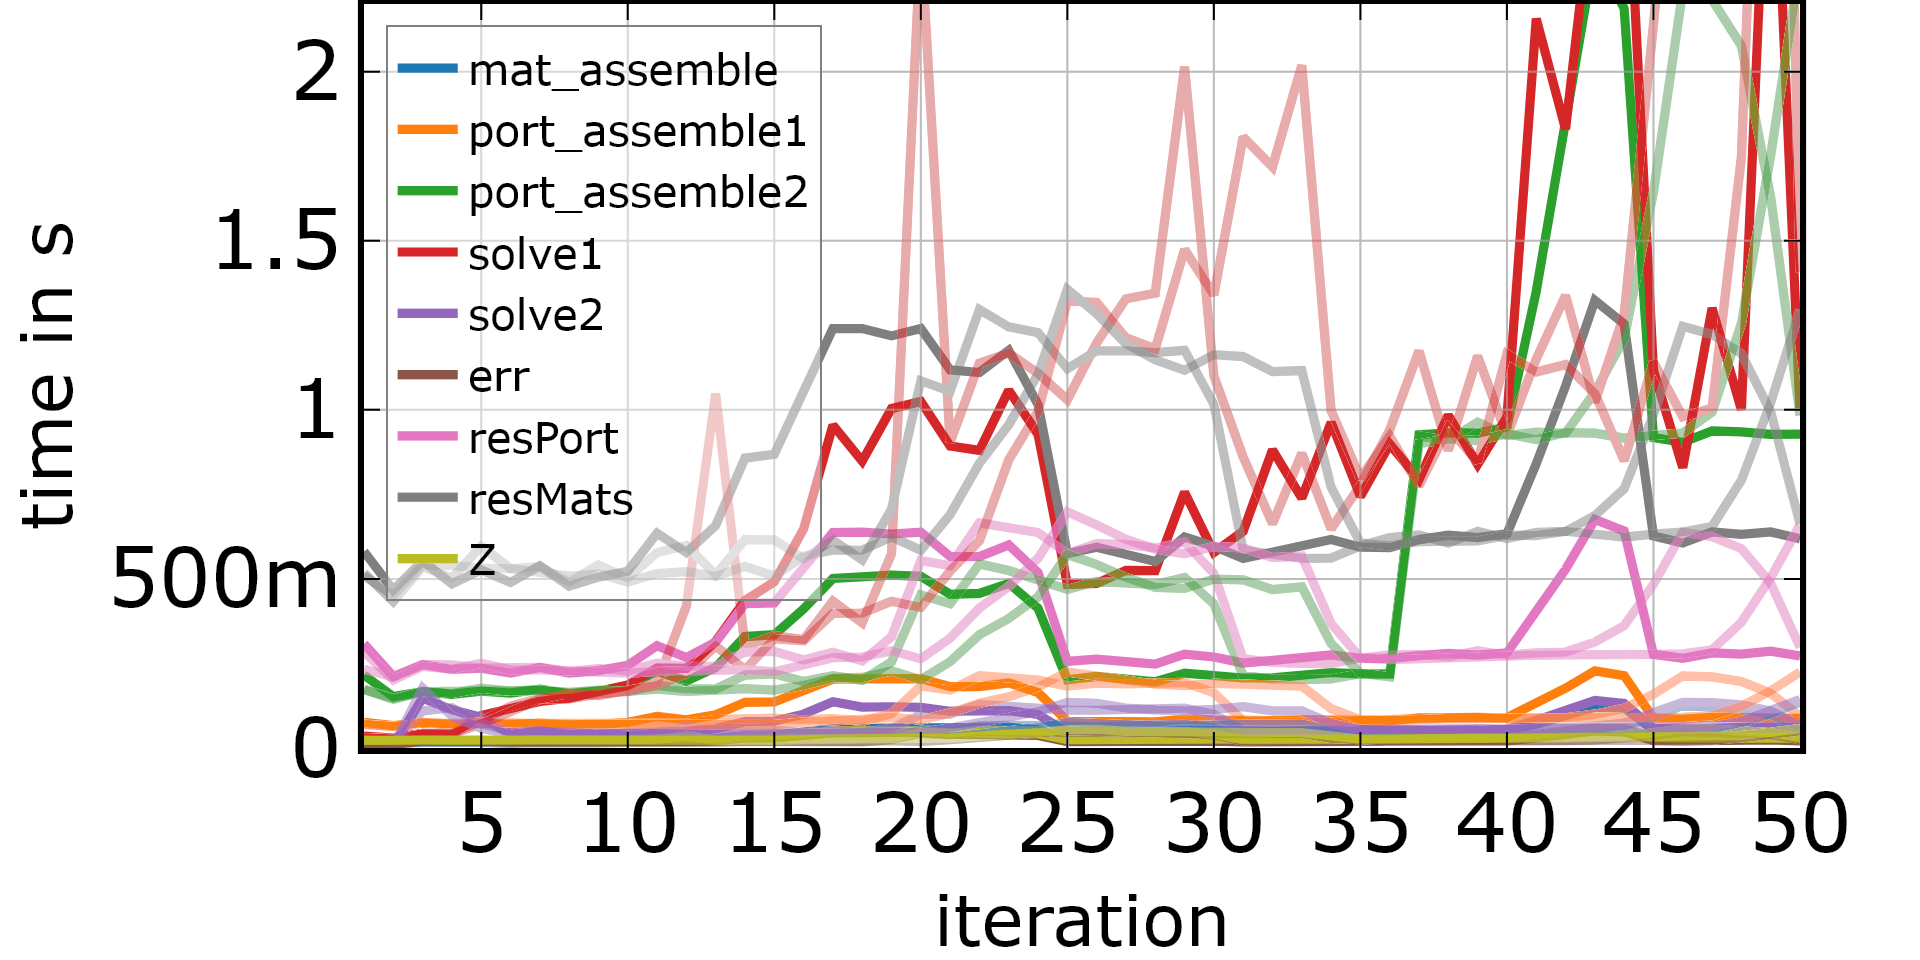
\includegraphics[width=0.5\textwidth]{CubeWire_time_merge1.PNG}
	\caption{Three runtimes for the Cubewire. The opaque lines show one run, the transparent ones two further ones. The increases at around iteration 20 and 40 are likely due to the cooling/turbo boost of the laptop, which can be confirmed by monitoring the task manager. Occasional spikes are distributed randomly, so likely caused by background processes. Important is the sudden increase of port-assemble2 at iteration 37 in all three runs. Also important is solve1, since it is the one which is increasing the quickest.}
	\label{}
\end{figure}


\begin{figure}[h]
	\centering
	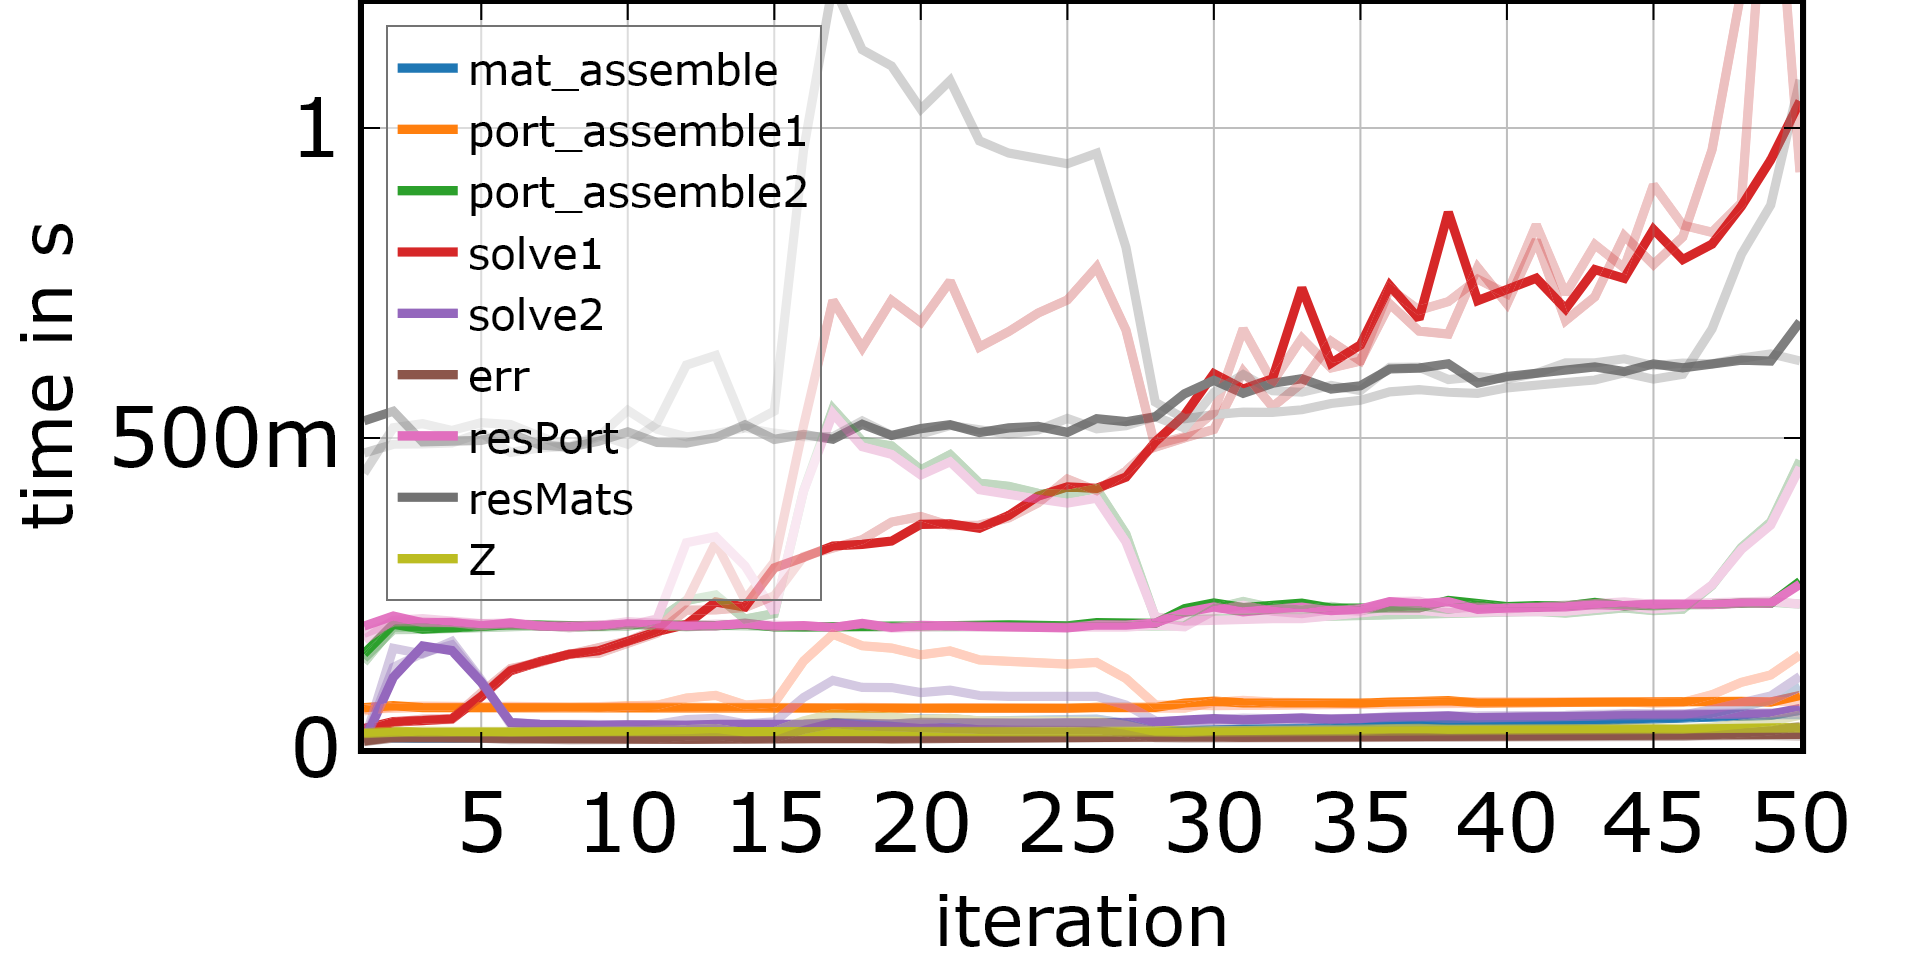
\includegraphics[width=0.5\textwidth]{sqav_time_merge1.PNG}
	\caption{Three runtimes for the square cavity. The opaque lines show one run, the transparent ones two further ones. Similar results as for the cube wire}
	\label{}
\end{figure}



\begin{figure}[h]
	\centering
	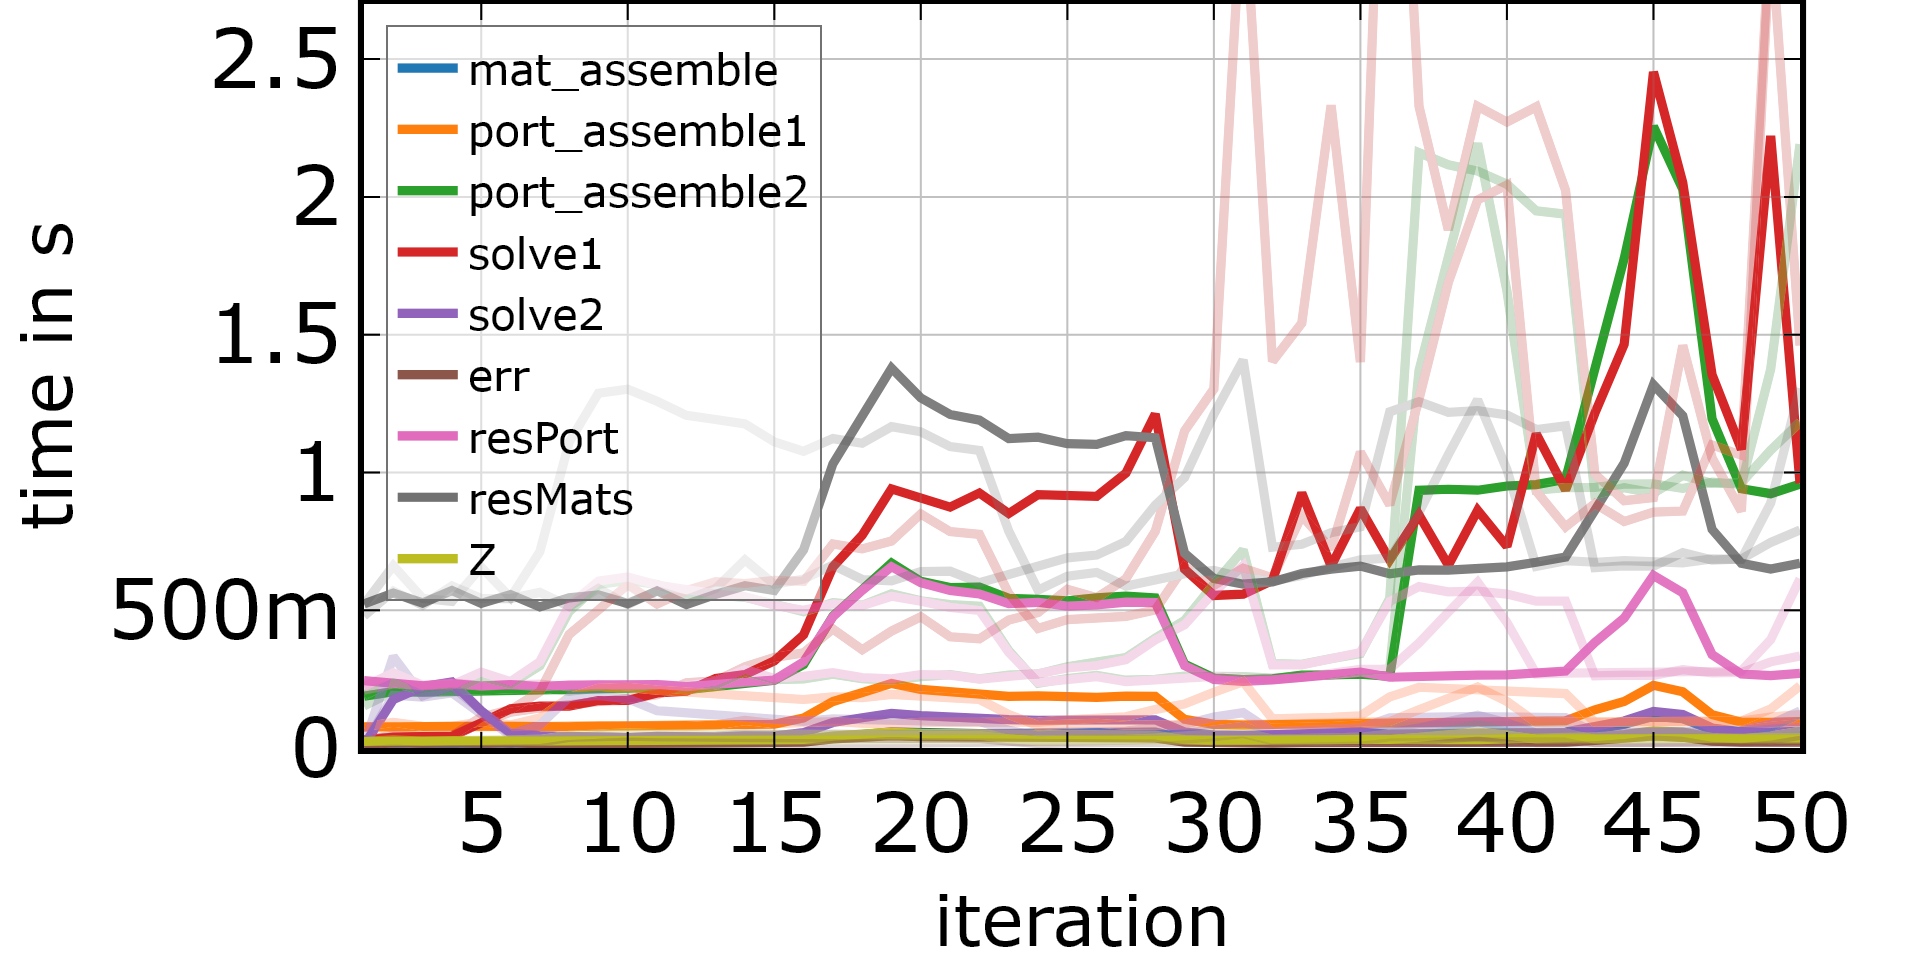
\includegraphics[width=0.5\textwidth]{const_time_merge1.PNG}
	\caption{Three runtimes for the constriction. The opaque lines show one run, the transparent ones two further ones. Similar results as for the cube wire. Here is also a sudden increase of port-assemble2 at iteration 37 in all three runs.59}
	\label{}
\end{figure}

\subsection{larger problem}
Time for FELIS Solution  545s for 100 evals -> 5450s for 1000 evals. MOR Took 2774s 


































